%
%  LSMR
% 
%  Created by Martell on 2012-08-15.
%  Copyright (c) 2012 UBC Fisheries Centre. All rights reserved.
%
\documentclass{beamer}
%\usetheme{Madrid} % My favorite!
%\usetheme{PaloAlto}
\usetheme{Goettingen}
%\usetheme{Hannover}
%\usetheme{Boadilla} % Pretty neat, soft color.
%\usetheme{default}
%\usetheme{Warsaw}
%\usetheme{Bergen} % This template has nagivation on the left
%\usetheme{Frankfurt} % Similar to the default 
%with an extra region at the top.
%\usecolortheme{seahorse} % Simple and clean template
%\usecolortheme{beaver}
%\usetheme{Darmstadt} % not so good
% Uncomment the following line if you want %
% page numbers and using Warsaw theme%
% \setbeamertemplate{footline}[page number]
%\setbeamercovered{transparent}
\setbeamercovered{invisible}
% To remove the navigation symbols from 
% the bottom of slides%
\setbeamertemplate{navigation symbols}{} 
%
\usepackage{color}
\usepackage{graphicx}
%\usepackage{bm}         % For typesetting bold math (not \mathbold)
%\logo{\includegraphics[height=0.6cm]{yourlogo.eps}}
%

%\definecolor{bottomcolour}{rgb}{0.32,0.3,0.38}
%\definecolor{middlecolour}{rgb}{0.08,0.08,0.16}
%\setbeamerfont{title}{size=\Huge}
%\setbeamercolor{structure}{fg=white}
%\setbeamertemplate{frametitle}[default][center]
%
%\setbeamercolor{normal text}{bg=black, fg=white}
%\setbeamertemplate{background canvas}[vertical shading]
%[bottom=bottomcolour, middle=middlecolour, top=black]
%
%\setbeamertemplate{itemize item}{\lower3pt\hbox{\Large\textbullet}}
%\setbeamerfont{frametitle}{size=\huge}
%

\title[LSMR]{A length-structured mark-recapture model}
\subtitle{Estimation of humpback chub abundance in the Grand Canyon using LSMR}
\author{Steven Martell}
\institute[UBC]
{
University of British Columbia \\
\medskip
{\emph{martell.steve@gmail.com}}
}
\date{\today}
% \today will show current date. 
% Alternatively, you can specify a date.
%
\begin{document}
%
\begin{frame}
\titlepage
\end{frame}
%
%
\section[Introduction]{Introduction} % (fold)
\label{sec:introduction}
%
\begin{frame}
\frametitle{Motivation}
\begin{block}
{Why a length-structured model?}
\begin{itemize}
	\item Assigning age from length implies growth is known.
	\item ASMR is an observation error only model; uncertainty under-estimated.
	\item Information on individuals $<$ 150mm (100mm) is discarded.
\end{itemize}

\end{block}
\end{frame}

\begin{frame}
	\frametitle{Introduction}
	\only<1>
	{
		\begin{itemize}
			\item Majority of HBC captured, tagged, and recaptured are sampled by hoop nets.
			\item Since 1989, there have been 81,812 capture \& recapture records of HBC.
			\item 67,296 captured in hoop nets, 4,306 in tramel nets, and 9,043 detections.
			\item Catch from hoop and tramel nets were disaggregated due to differences in sampling effort.
			\item Minimum size of tagging was 150mm TL, and in recent years reduced to 100mm TL.
		\end{itemize}
	}
	\only<2>
	{
		\begin{block}{Model Structure}
			\begin{itemize}
				\item Data: catch-at-length (marked \& unmarked), annual growth increments.
				\item Parameters: Initial lengths, length \& abundance of new recruits, capture probability, natural mortality.
				\item Psuedocode:
					\begin{enumerate}
						\item Construct size-transition matrixes from growth increment data.
						\item Initialize No.-at-length \& annual recruits-at-length.
						\item Survive \& grow fish each year.
						\item Compute marked \& unmarked catch-at-length.
						\item Minimize -log negative binomial likelihood.
						\item Use Metropolis-Hastings to sample joint posterior distribution.
					\end{enumerate}
			\end{itemize}
		\end{block}
	}
\end{frame}


% section introduction (end)
%%
%%
\section[Data]{Input Data} % (fold)
\label{sec:data}

\subsection{Size Transition} % (fold)
\label{sub:size_transition}


\begin{frame}
	\frametitle{Size transition probabilities}
	\only<1>
	{
		\begin{block}{Psuedocode:}
			\begin{enumerate}
				\item Extract annual growth increments for individuals capture \& recaptured in subsequent year.
				\item Estimate annual growth parameters in a Bayesian hierarchical model.
				\item Construct size-transition matrix using parametric uncertainty and measurement error with $\sigma=9.4$mm.
			\end{enumerate}
		\end{block}
	}
	
	\only<2>
	{
		 \begin{figure}[htbp]
		 	\centering
		 		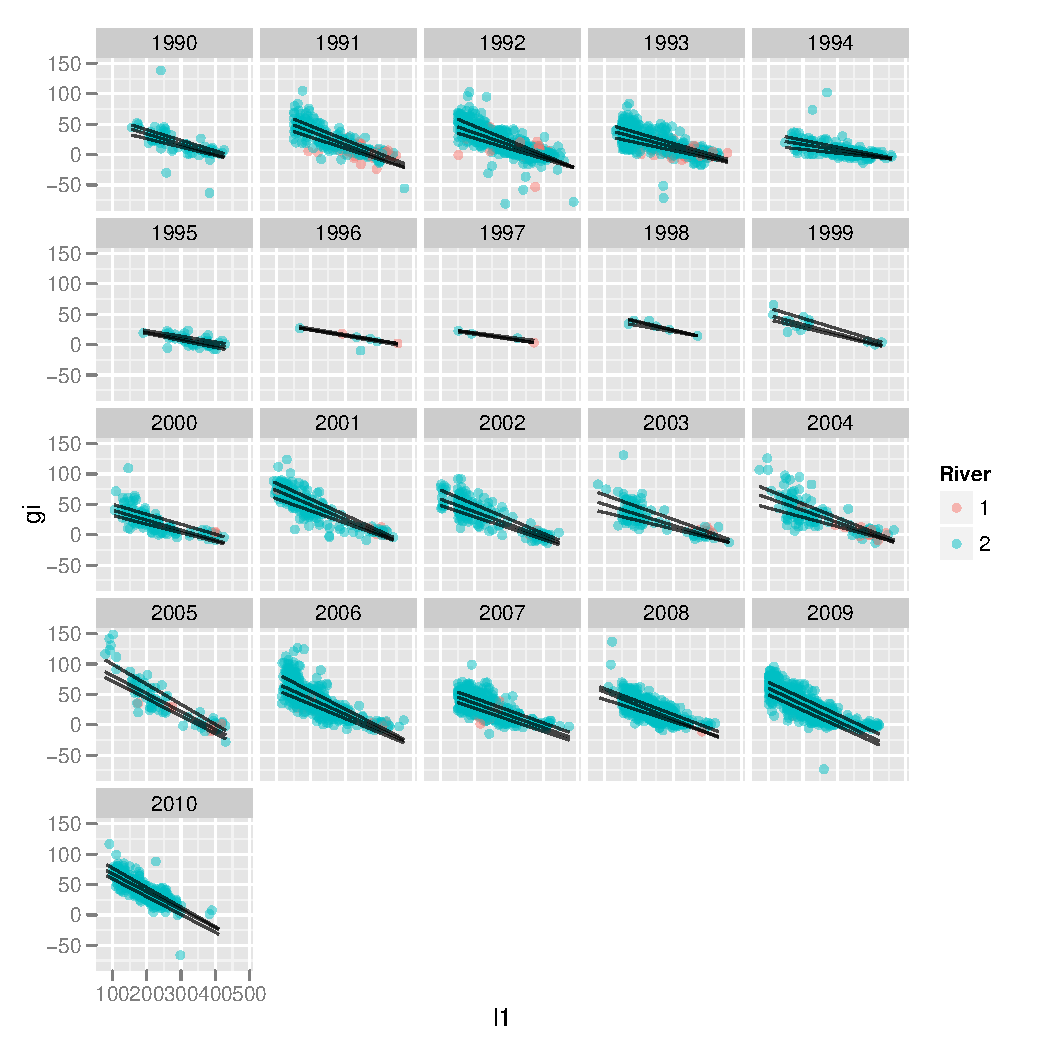
\includegraphics[height=2.8in]{../../FIGS/LSMR/fig:AnnualGrowthIncrements.pdf}
			\caption{Annual growth increments for individuals marked in year $t$ and recaptured in year $t+1$ in LCR (blue) and COL (red).}
		 	\label{fig:FIGS_LSMR_fig:AnnualGrowthIncrements}
		 \end{figure}
	}
	\only<3>
	{
		\begin{figure}[htbp]
			\centering
				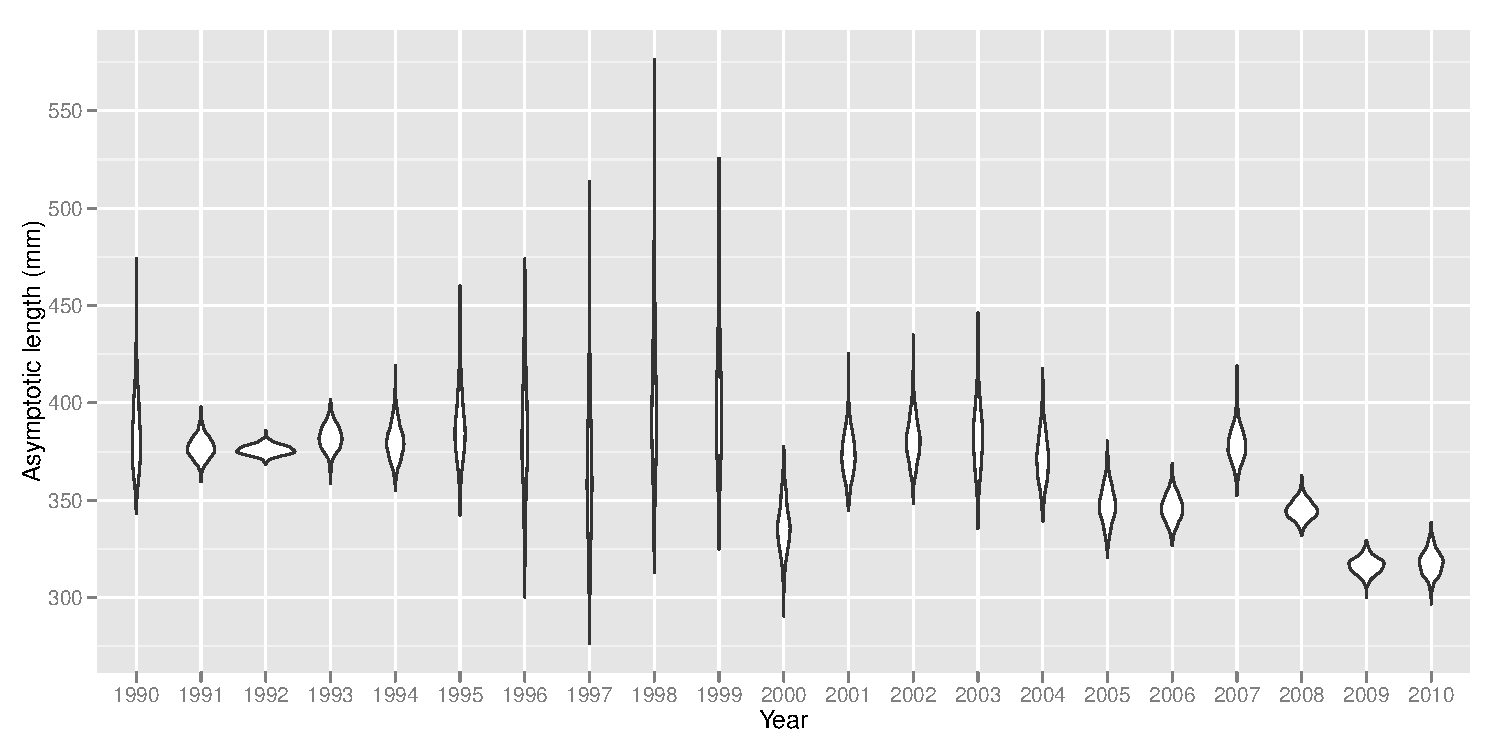
\includegraphics[width=2.8in]{../../FIGS/LSMR/fig:LinfPosteriors.pdf}\\
				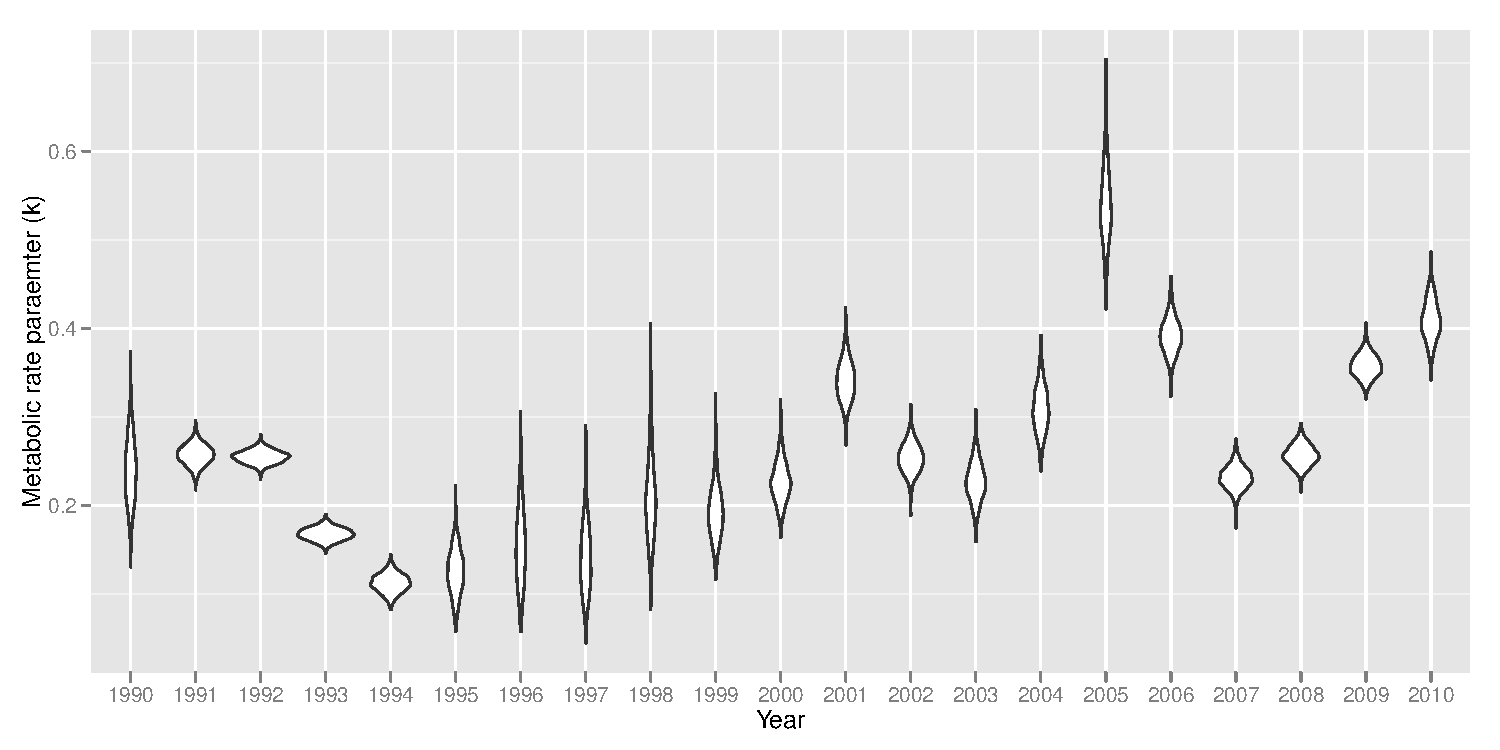
\includegraphics[width=2.8in]{../../FIGS/LSMR/fig:kPosteriors.pdf}
			\caption{Marginal posterior distributions for growth parameters $l_\infty$ and $k$.}
			\label{fig:FIGS_LSMR_fig:LinfPosteriors}
		\end{figure}
	}
	\only<4>
	{
		\begin{figure}[htbp]
			\centering
				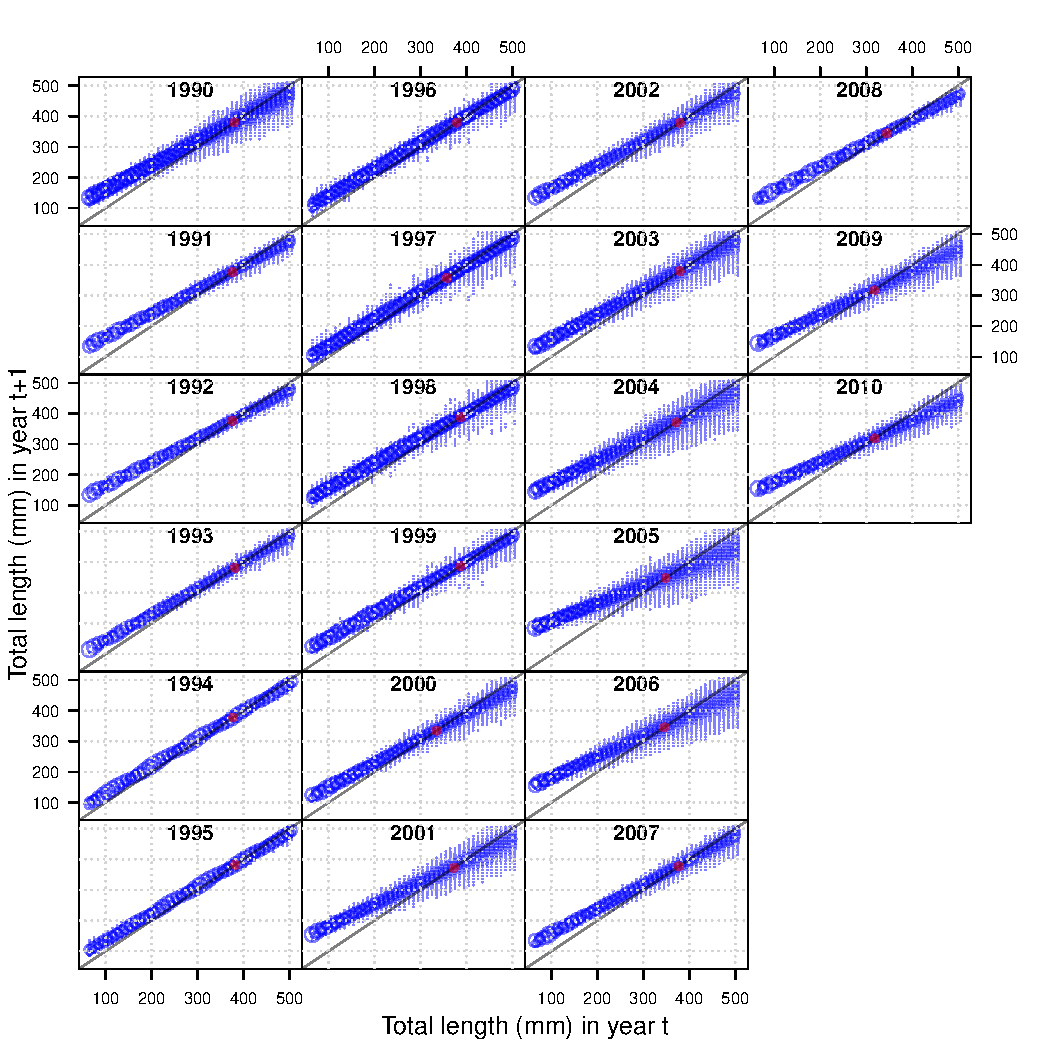
\includegraphics[height=3in]{../../FIGS/LSMR/fig:TransitionMatrix.pdf}
			\caption{Annual size transition matrix based on annual growth increments.}
			\label{fig:FIGS_LSMR_fig:TransitionMatrix}
		\end{figure}	
	}
\end{frame}
% subsection size_transition (end)

\subsection{Catch-at-length} % (fold)
\label{sub:catch_at_length}
\begin{frame}
	\frametitle{Catch-at-length}
	\begin{figure}[htbp]
		\centering
			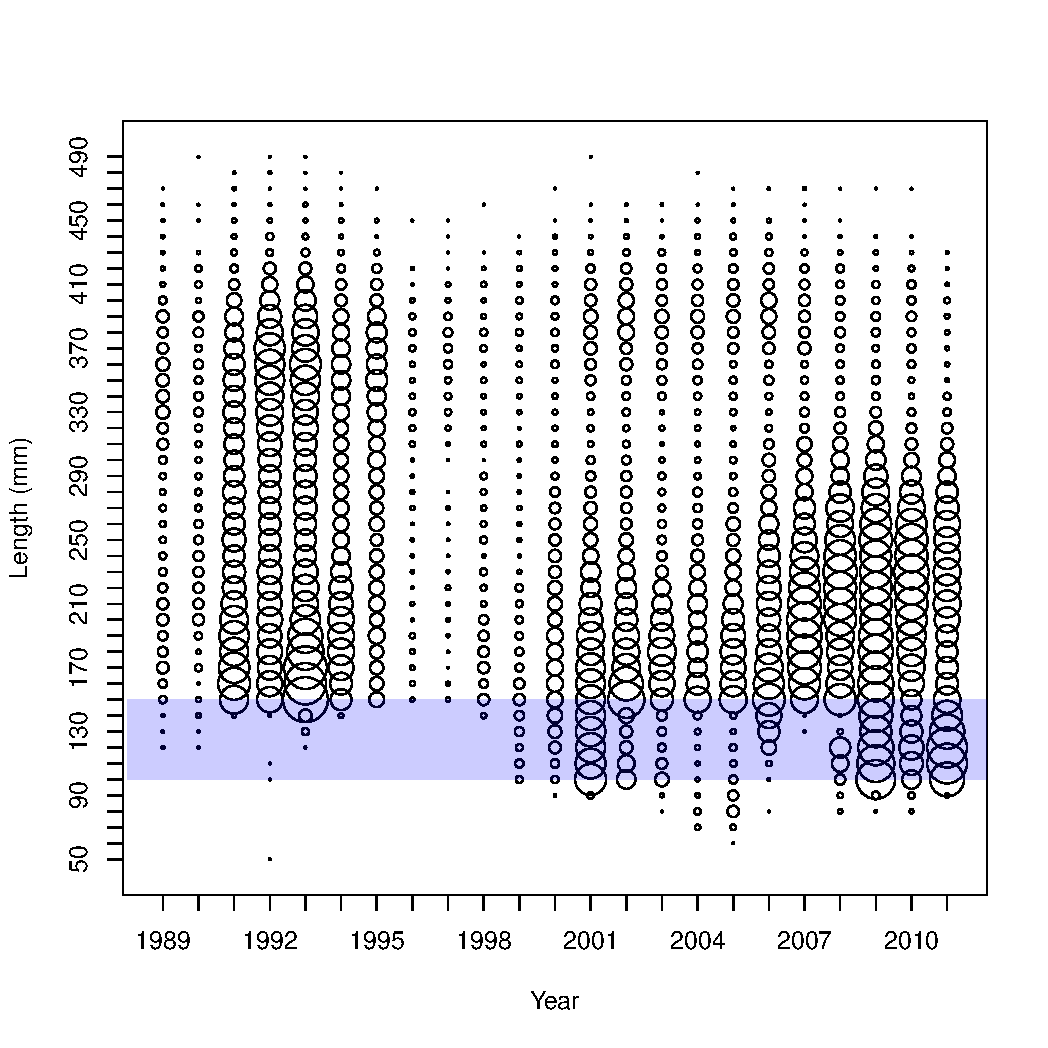
\includegraphics[height=2.6in]{../../FIGS/LSMR/fig:CaptureLFbubbles.pdf}
		\caption{Length frequencies for all gear types. Area of circle is proportional to abundance of measured fish, shaded region represents the 100-150 mm size interval.}
		\label{fig:FIGS_LSMR_fig:CaptureLFbubbles}
	\end{figure}
\end{frame}

\begin{frame}
	\frametitle{Catch-at-length: hoop nets}
	\begin{figure}[htbp]
		\centering
			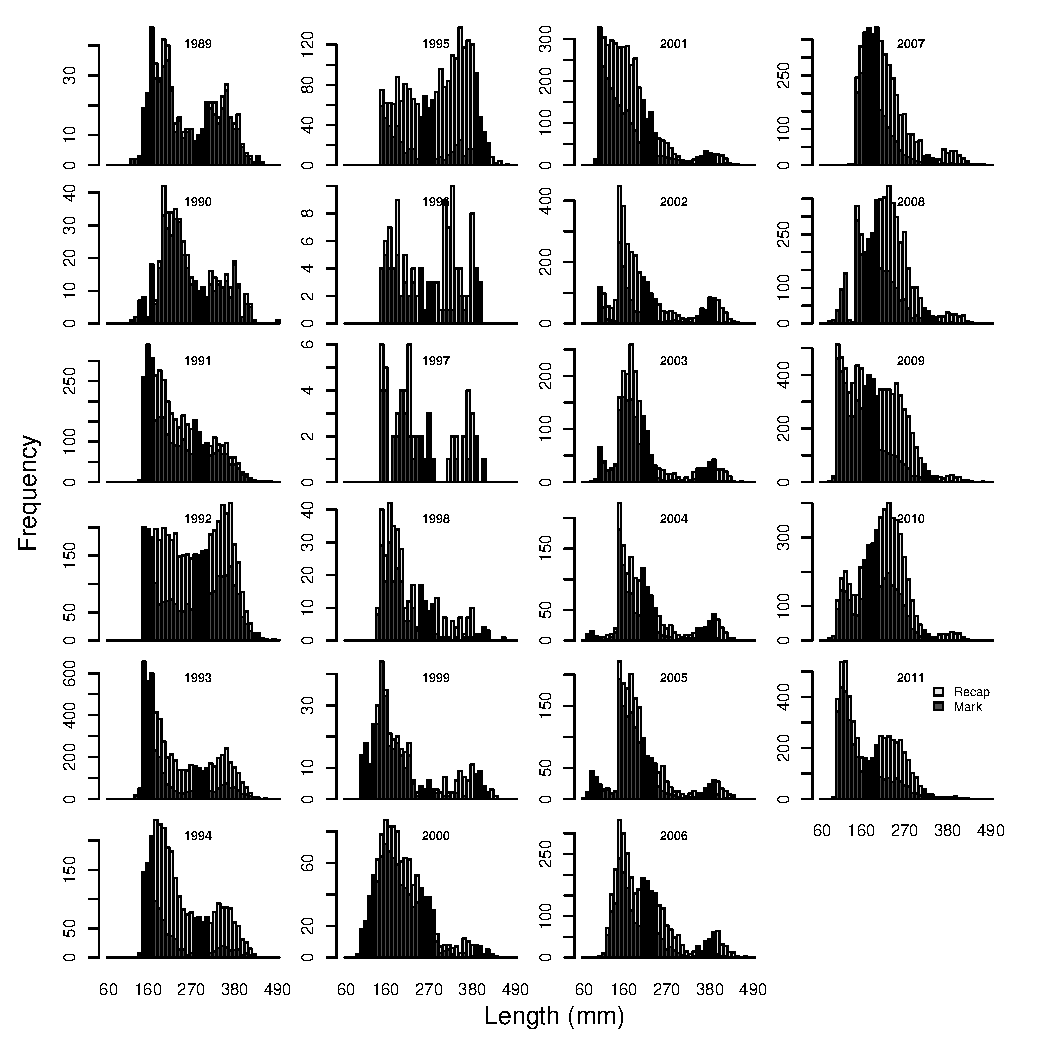
\includegraphics[height=2.6in]{../../FIGS/LSMR/fig:MarksAtLengthHOOP.pdf}
		\caption{New marks (dark bars) and recapture marks (light bars) of HBC using hoop nets (all sizes \& bait) in the LCR and COR.}
		\label{fig:FIGS_LSMR_fig:MarksAtLengthHOOP}
	\end{figure}
	
\end{frame}
\begin{frame}
	\frametitle{Catch-at-length: tramel nets}
	\begin{figure}[htbp]
		\centering
			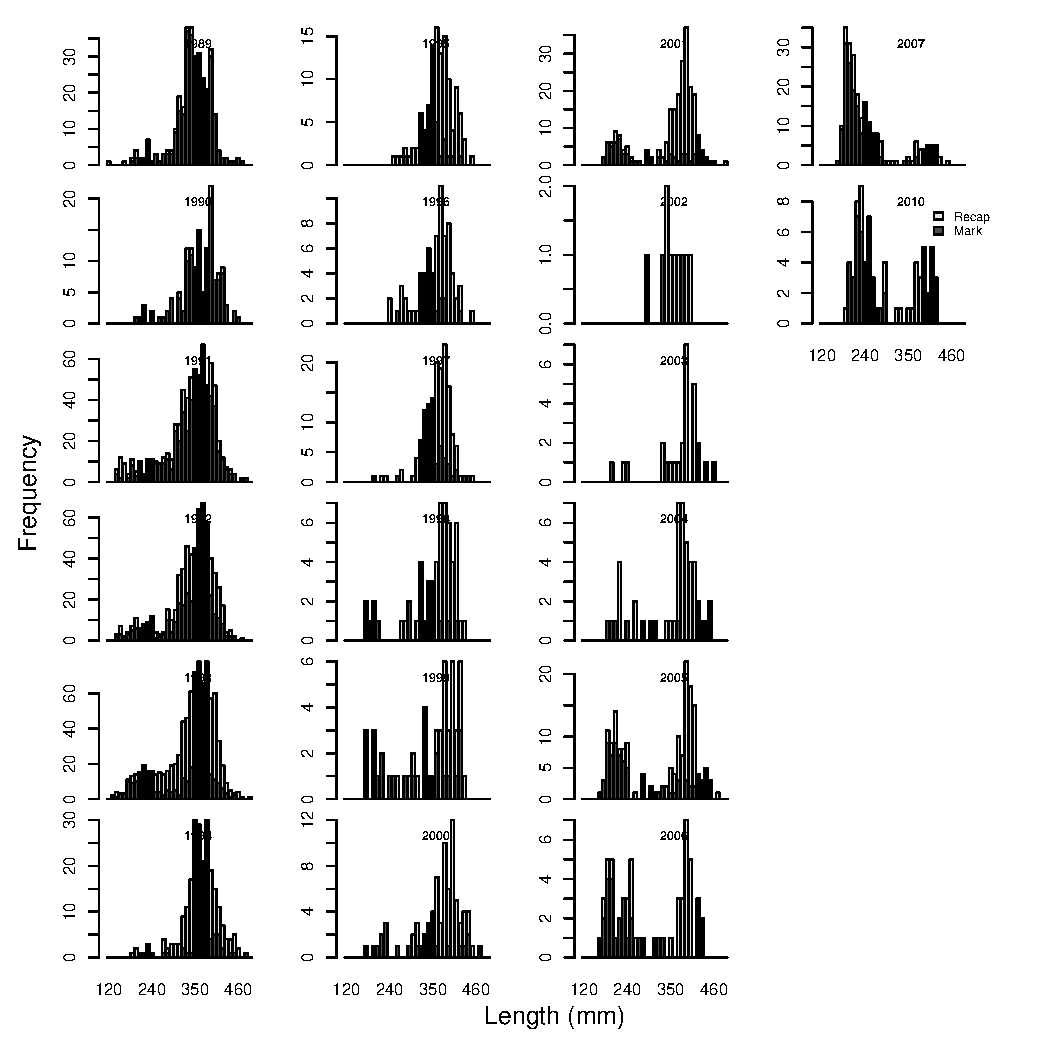
\includegraphics[height=2.6in]{../../FIGS/LSMR/fig:MarksAtLengthGILL.pdf}
		\caption{New marks (dark bars) and recapture marks (light bars) of HBC using tramel nets (all sizes \& bait) in the LCR and COR.}
		\label{fig:FIGS_LSMR_fig:MarksAtLengthGILL}
	\end{figure}
\end{frame}
% subsection catch_at_length (end)

% section data (end)
%%
%%
\section{LSRM Model} % (fold)
\label{sec:lsrm_model}
\begin{frame}
	\frametitle{Length-structured mark-recapture model}
	\only<1>
	{
		\begin{block}{Objective}
			Fit a length-based model to capture and recapture-at-length data, while jointly estimating abundance, growth and survival rates.
		\end{block}
		
		\begin{block}{Difference between LSMR and ASMR}
			\begin{itemize}
				\item Forward reconstruction of unmarked individuals.
				\item Estimate size-based capture probabilities.
			\end{itemize}
		\end{block}
	}
	\only<2>
	{
		\begin{block} {Dynamics of numbers-at-length}
			\begin{itemize}
				\item Let $\vec{N}$ = vector of individuals at length intervals $l$,
				\item let $\vec{M}$ = vector of size $l$ specific survival rates,
				\item let $P$ = a size transition matrix from size $l$ to $l'$, and
				\item let $\vec{R}$ = vector of new recruits at length intervals $l$.
			\end{itemize}
			Then the number of individuals at the next time step is given by:
			\[ \vec{N}_{t+\Delta t} = \vec{N}_t \vec{M} P_{l,l'} + \vec{R}_t\]
			
		\end{block}
	}
	\only<3>
	{
		\begin{block} {Predicted catch-at-length}
			\begin{itemize}
				\item Let $\vec{\pi}$ = a vector of size-specific capture probabilities,
				\item let $\vec{N}$ = vector of individuals at length intervals $l$
			\end{itemize}
			Then the predicted catch-at-length in year $t$ is given by:
			\[
				\vec{C}_t  = \vec{\pi}_t \vec{N}_t
			\]
			
		\end{block}
	}
	
	
\end{frame}
% section lsrm_model (end)

\section{Simulation testing} % (fold)
\label{sec:simulation_testing}


\begin{frame}
	\frametitle{Simulation testing}
	\begin{block} {Objective}
		Use simulated data to demonstrate estimability of model parameters.
	\end{block}
	\begin{block}{Scenarios}
		\begin{enumerate}
			\item Perfect information (no observation errors).
			\item Mixed error: error in size-specific capture probabilities.
		\end{enumerate}
	\end{block}
\end{frame}

\begin{frame}{Simulation (Scenario 1)}
	\begin{figure}[htbp]
		\centering
			\includegraphics[height=1.4in]{../../FIGS/LSMR/SIMa/fig:LSRM1.png}
			\includegraphics[height=1.4in]{../../FIGS/LSMR/SIMa/fig:LSRM2.png}\\
			\includegraphics[height=1.4in]{../../FIGS/LSMR/SIMa/fig:LSRM3.png}
			\includegraphics[height=1.4in]{../../FIGS/LSMR/SIMa/fig:LSRM4.png}
		\caption{MLE results with perfect information.}
		\label{fig:FIGS_LSMR_SIMa_fig:LSRM1}
	\end{figure}
\end{frame}

\begin{frame}{Size composition (Tramel net, Scenario 1)}
	\only<1>
	{
		\begin{figure}[htbp]
			\centering
				\includegraphics[height=2.8in]{../../FIGS/LSMR/SIMa/fig:LSRM8.png}
			\caption{Simulated (shaded) and estimated predicted total catch.}
			\label{fig:FIGS_LSMR_SIMa_fig:LSRM8}
		\end{figure}
	}
	\only<2>
	{
	\frametitle{Size composition (Hoop net, Scenario 1)}
		\begin{figure}[htbp]
			\centering
				\includegraphics[height=2.8in]{../../FIGS/LSMR/SIMa/fig:LSRM11.png}
			\caption{Simulated (shaded) and estimated predicted total catch.}
			\label{fig:FIGS_LSMR_SIMa_fig:LSRM11}
		\end{figure}
	}
	
\end{frame}


\begin{frame}{Simulation (Scenario 2)}
	\begin{figure}[htbp]
		\centering
			\includegraphics[height=1.4in]{../../FIGS/LSMR/SIMb/fig:LSRM1.png}
			\includegraphics[height=1.4in]{../../FIGS/LSMR/SIMb/fig:LSRM2.png}\\
			\includegraphics[height=1.4in]{../../FIGS/LSMR/SIMb/fig:LSRM3.png}
			\includegraphics[height=1.4in]{../../FIGS/LSMR/SIMb/fig:LSRM4.png}
		\caption{MLE results with $\sigma_\delta = 0.2$.}
		\label{fig:FIGS_LSMR_SIMb_fig:LSRM1}
	\end{figure}
	
		
\end{frame}

\begin{frame}{Size composition (Tramel net, Scenario 2)}
	\only<1>
	{
		\begin{figure}[htbp]
			\centering
				\includegraphics[height=2.8in]{../../FIGS/LSMR/SIMb/fig:LSRM8.png}
			\caption{Simulated (shaded) and estimated predicted total catch.}
			\label{fig:FIGS_LSMR_SIMb_fig:LSRM8}
		\end{figure}
	}
	\only<2>
	{
	\frametitle{Size composition (Hoop net, Scenario 2)}
		\begin{figure}[htbp]
			\centering
				\includegraphics[height=2.8in]{../../FIGS/LSMR/SIMb/fig:LSRM11.png}
			\caption{Simulated (shaded) and estimated predicted total catch.}
			\label{fig:FIGS_LSMR_SIMb_fig:LSRM11}
		\end{figure}
	}
	
\end{frame}

% section simulation_testing (end)

\section[Grand Canyon]{Application to Grand Canyon HBC} % (fold)
\label{sec:application_to_grand_canyon_hbc}
\begin{frame}
	\frametitle{Fitting LSMR to Grand Canyon data}
	\begin{block}{Run Scenarios:}
		\begin{enumerate}
			\item Logistic selectivity for both gears.
			\item Logistic for tramel nets, dome-shaped for hoop nets.
			\item Selectivity coefficients for hoop nets, logistic tramel nets.
			\item Selectivity coefficients for both gears.
		\end{enumerate}
		
	\end{block}
\end{frame}

\begin{frame}
	\frametitle{Run 1: Logistic selectivity}
	\begin{figure}[htbp]
		\centering
			\includegraphics[height=1.4in]{../../FIGS/LSMR/RUN1/fig:LSRM1.png}
			\includegraphics[height=1.4in]{../../FIGS/LSMR/RUN1/fig:LSRM2.png}\\
			\includegraphics[height=1.4in]{../../FIGS/LSMR/RUN1/fig:LSRM3.png}
			\includegraphics[height=1.4in]{../../FIGS/LSMR/RUN1/fig:LSRM5.png}
		\caption{Abundance, recruitment, capture probability, and selectivity.}
		\label{fig:FIGS_LSMR_RUN1_fig:LSRM1}
	\end{figure}
	
\end{frame}

\begin{frame}
	\frametitle{Run 2: Logistic \& dome-shaped selectivity}
	\begin{figure}[htbp]
		\centering
			\includegraphics[height=1.4in]{../../FIGS/LSMR/RUN2/fig:LSRM1.png}
			\includegraphics[height=1.4in]{../../FIGS/LSMR/RUN2/fig:LSRM2.png}\\
			\includegraphics[height=1.4in]{../../FIGS/LSMR/RUN2/fig:LSRM3.png}
			\includegraphics[height=1.4in]{../../FIGS/LSMR/RUN2/fig:LSRM5.png}
		\caption{Abundance, recruitment, capture probability, and selectivity.}
		\label{fig:FIGS_LSMR_RUN2_fig:LSRM1}
	\end{figure}
	
\end{frame}

\begin{frame}
	\frametitle{Run 3: Selectivity coefficients}
	\begin{figure}[htbp]
		\centering
			\includegraphics[height=1.4in]{../../FIGS/LSMR/RUN3/fig:LSRM1.png}
			\includegraphics[height=1.4in]{../../FIGS/LSMR/RUN3/fig:LSRM2.png}\\
			\includegraphics[height=1.4in]{../../FIGS/LSMR/RUN3/fig:LSRM3.png}
			\includegraphics[height=1.4in]{../../FIGS/LSMR/RUN3/fig:LSRM5.png}
		\caption{Abundance, recruitment, capture probability, and selectivity.}
		\label{fig:FIGS_LSMR_RUN3_fig:LSRM1}
	\end{figure}
	
\end{frame}


% section application_to_grand_canyon_hbc (end)


% 
\section{Resources} % (fold)
\label{sec:resources}


\begin{frame}
	\frametitle{More details ...}
	
	Code @:
	\url{https://github.com/smartell/LSMR}
\end{frame}
% section resources (end) 



 
\begin{frame}
\centerline{The End}
\end{frame}
% End of slides
\end{document}

